\documentclass[../Article_Sensitivity_Analsysis.tex]{subfiles}
\graphicspath{{\subfix{../Figures/}}}
\begin{document}
	
	\label{CH: Results}
	
	To identify the global solution of Equations \ref{EQ:Formulation}, the optimization problem is solved multiple times, with each run starting from a random initial solution sampled from a uniform distribution. Figure \ref{fig:scatter} compares the initial and final values of the cost function across multiple optimization runs for all cases. The solution with the lowest cost function value is considered the global solution for each case.
	
	\begin{figure}[h!]
		\centering
		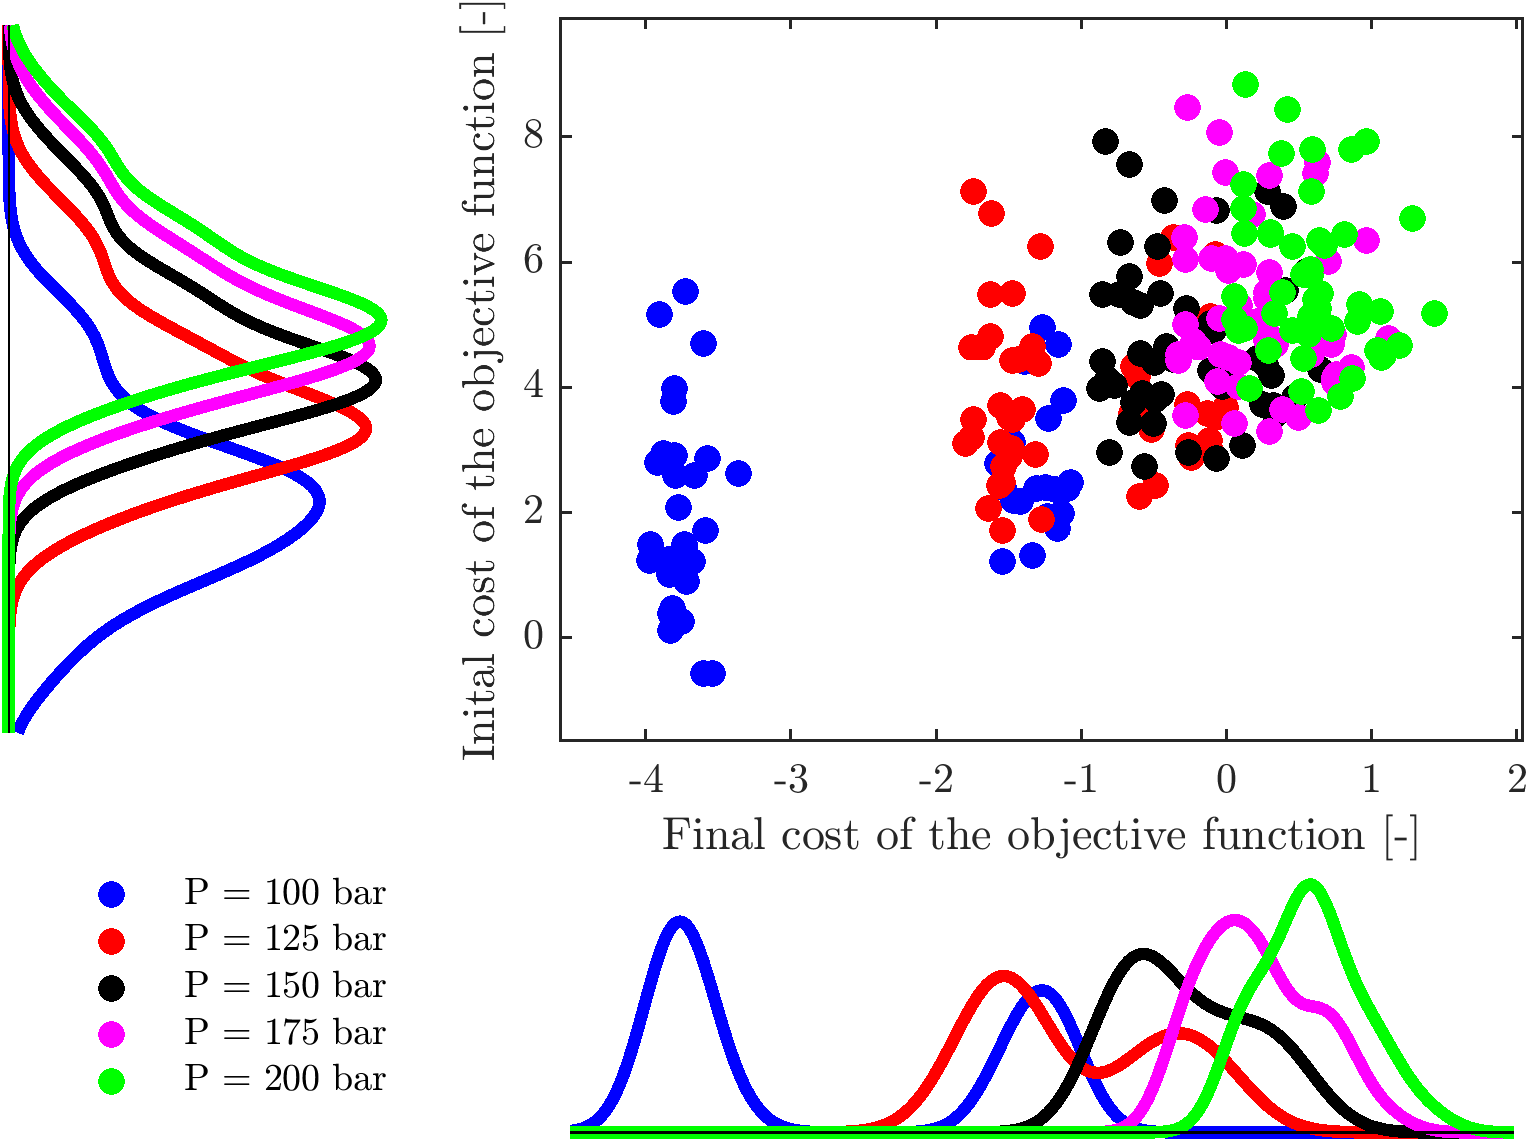
\includegraphics[width=\columnwidth]{Figures/Results/scatter.png}	
		\caption{Initial vs final values of the cost function}
		\label{fig:scatter}
	\end{figure}
	
	From the Figure \ref{fig:scatter}, show an existence of a global solution for the case of $P=100$ bar because all the optimization runs converged to the same point. For this case, the obtained final value of the objective function is the smallest, which indicate the at this an experiment for the highest discrimination. All the other cases are characterized by higher final values of the objective function compare to the of $P=100$ bar. By close analysis of the Figure \ref{fig:scatter}, it can be observed that the obtained solution for case of $P=125$ bar are characterized by the highest final value of the objective function. In this case, the discrimination between models is the most challenging. The optimal profiles of the controls for each case are presented in Figures  \ref{fig:Profiles_T} and \ref{fig:Profiles_F}.
	
	\begin{figure}[h!]
		\centering
		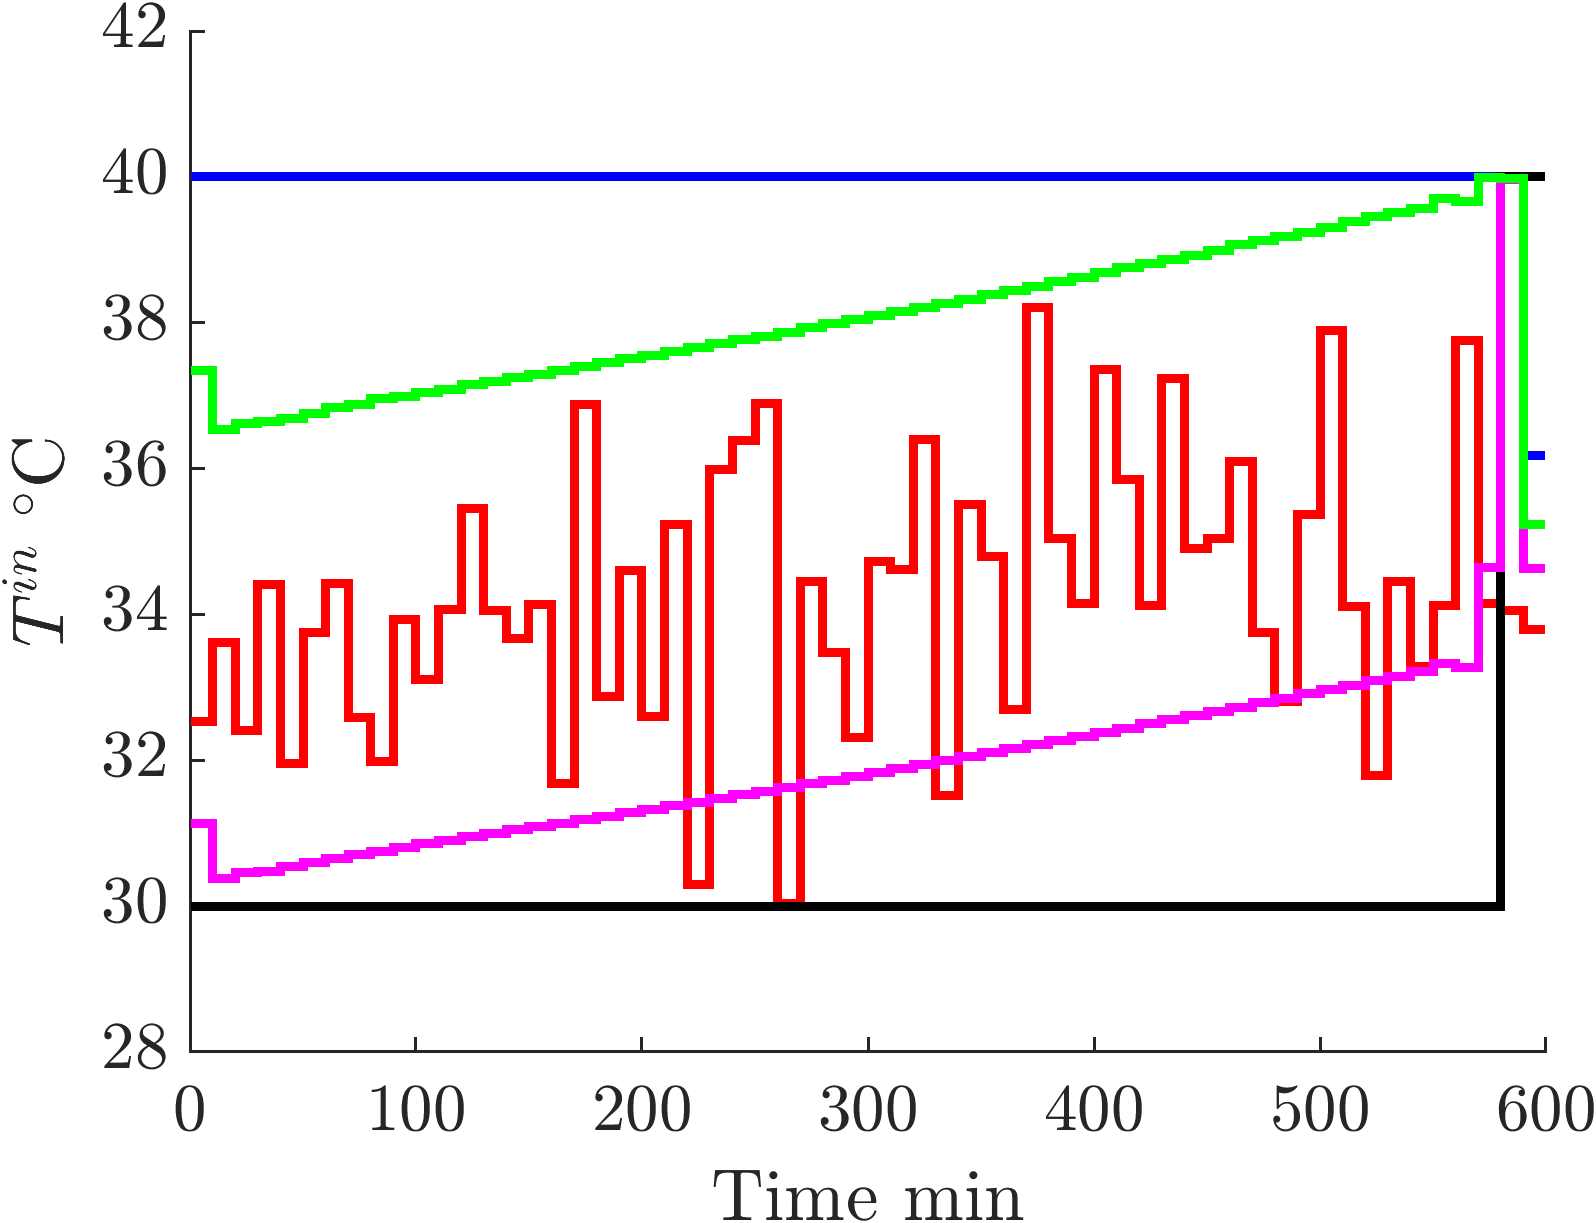
\includegraphics[width=0.8\columnwidth]{Figures/Results/Profiles_T.png}	
		\caption{Optimal profiles of the inlet temperature}
		\label{fig:Profiles_T}
	\end{figure}
	
	The obtained profiles of the inlet temperature differ from each other depending on the case. For $P = 100$ and $P = 150$ bar, the temperature stay constant all the time and change in the last period.
	
	\begin{figure}[h!]
		\centering
		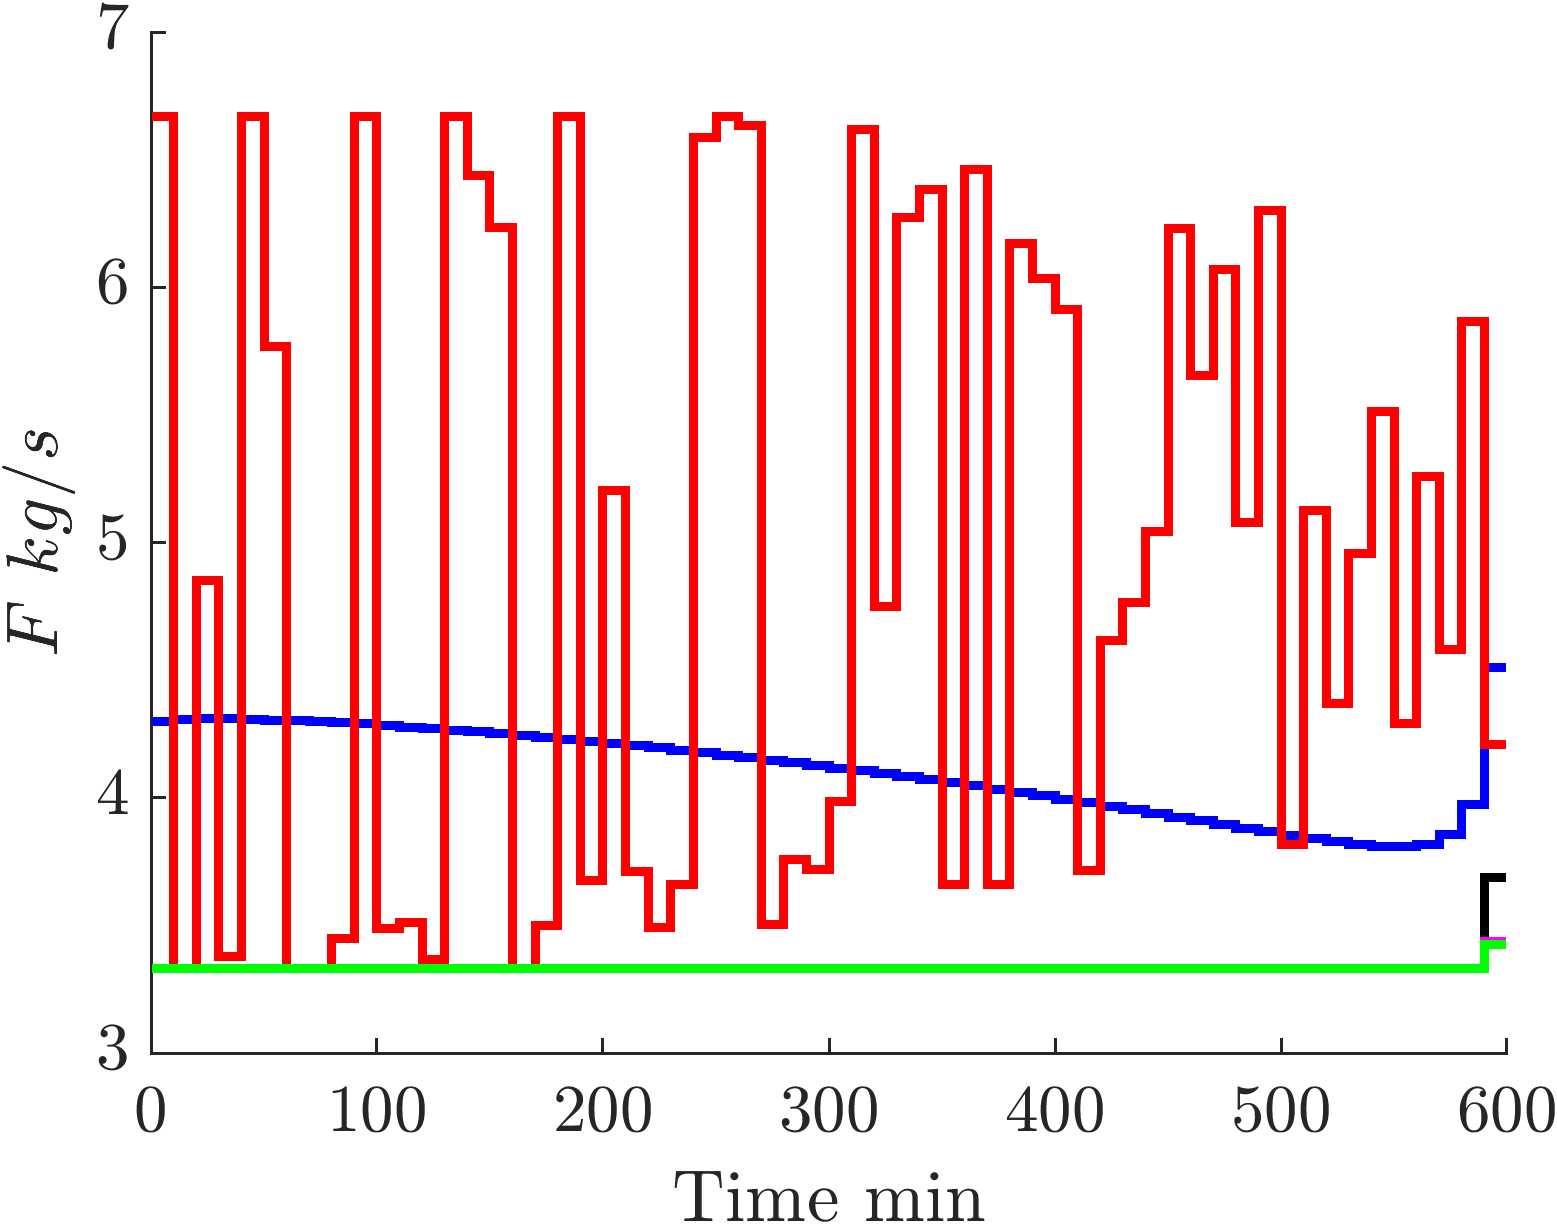
\includegraphics[width=0.8\columnwidth]{Figures/Results/Profiles_F.png}	
		\caption{Optimal profiles of the mass flow rate}
		\label{fig:Profiles_F}
	\end{figure}
	
	The obtained yield profiles are shown in Figure 
	
	\begin{figure}[h!]
		\centering
		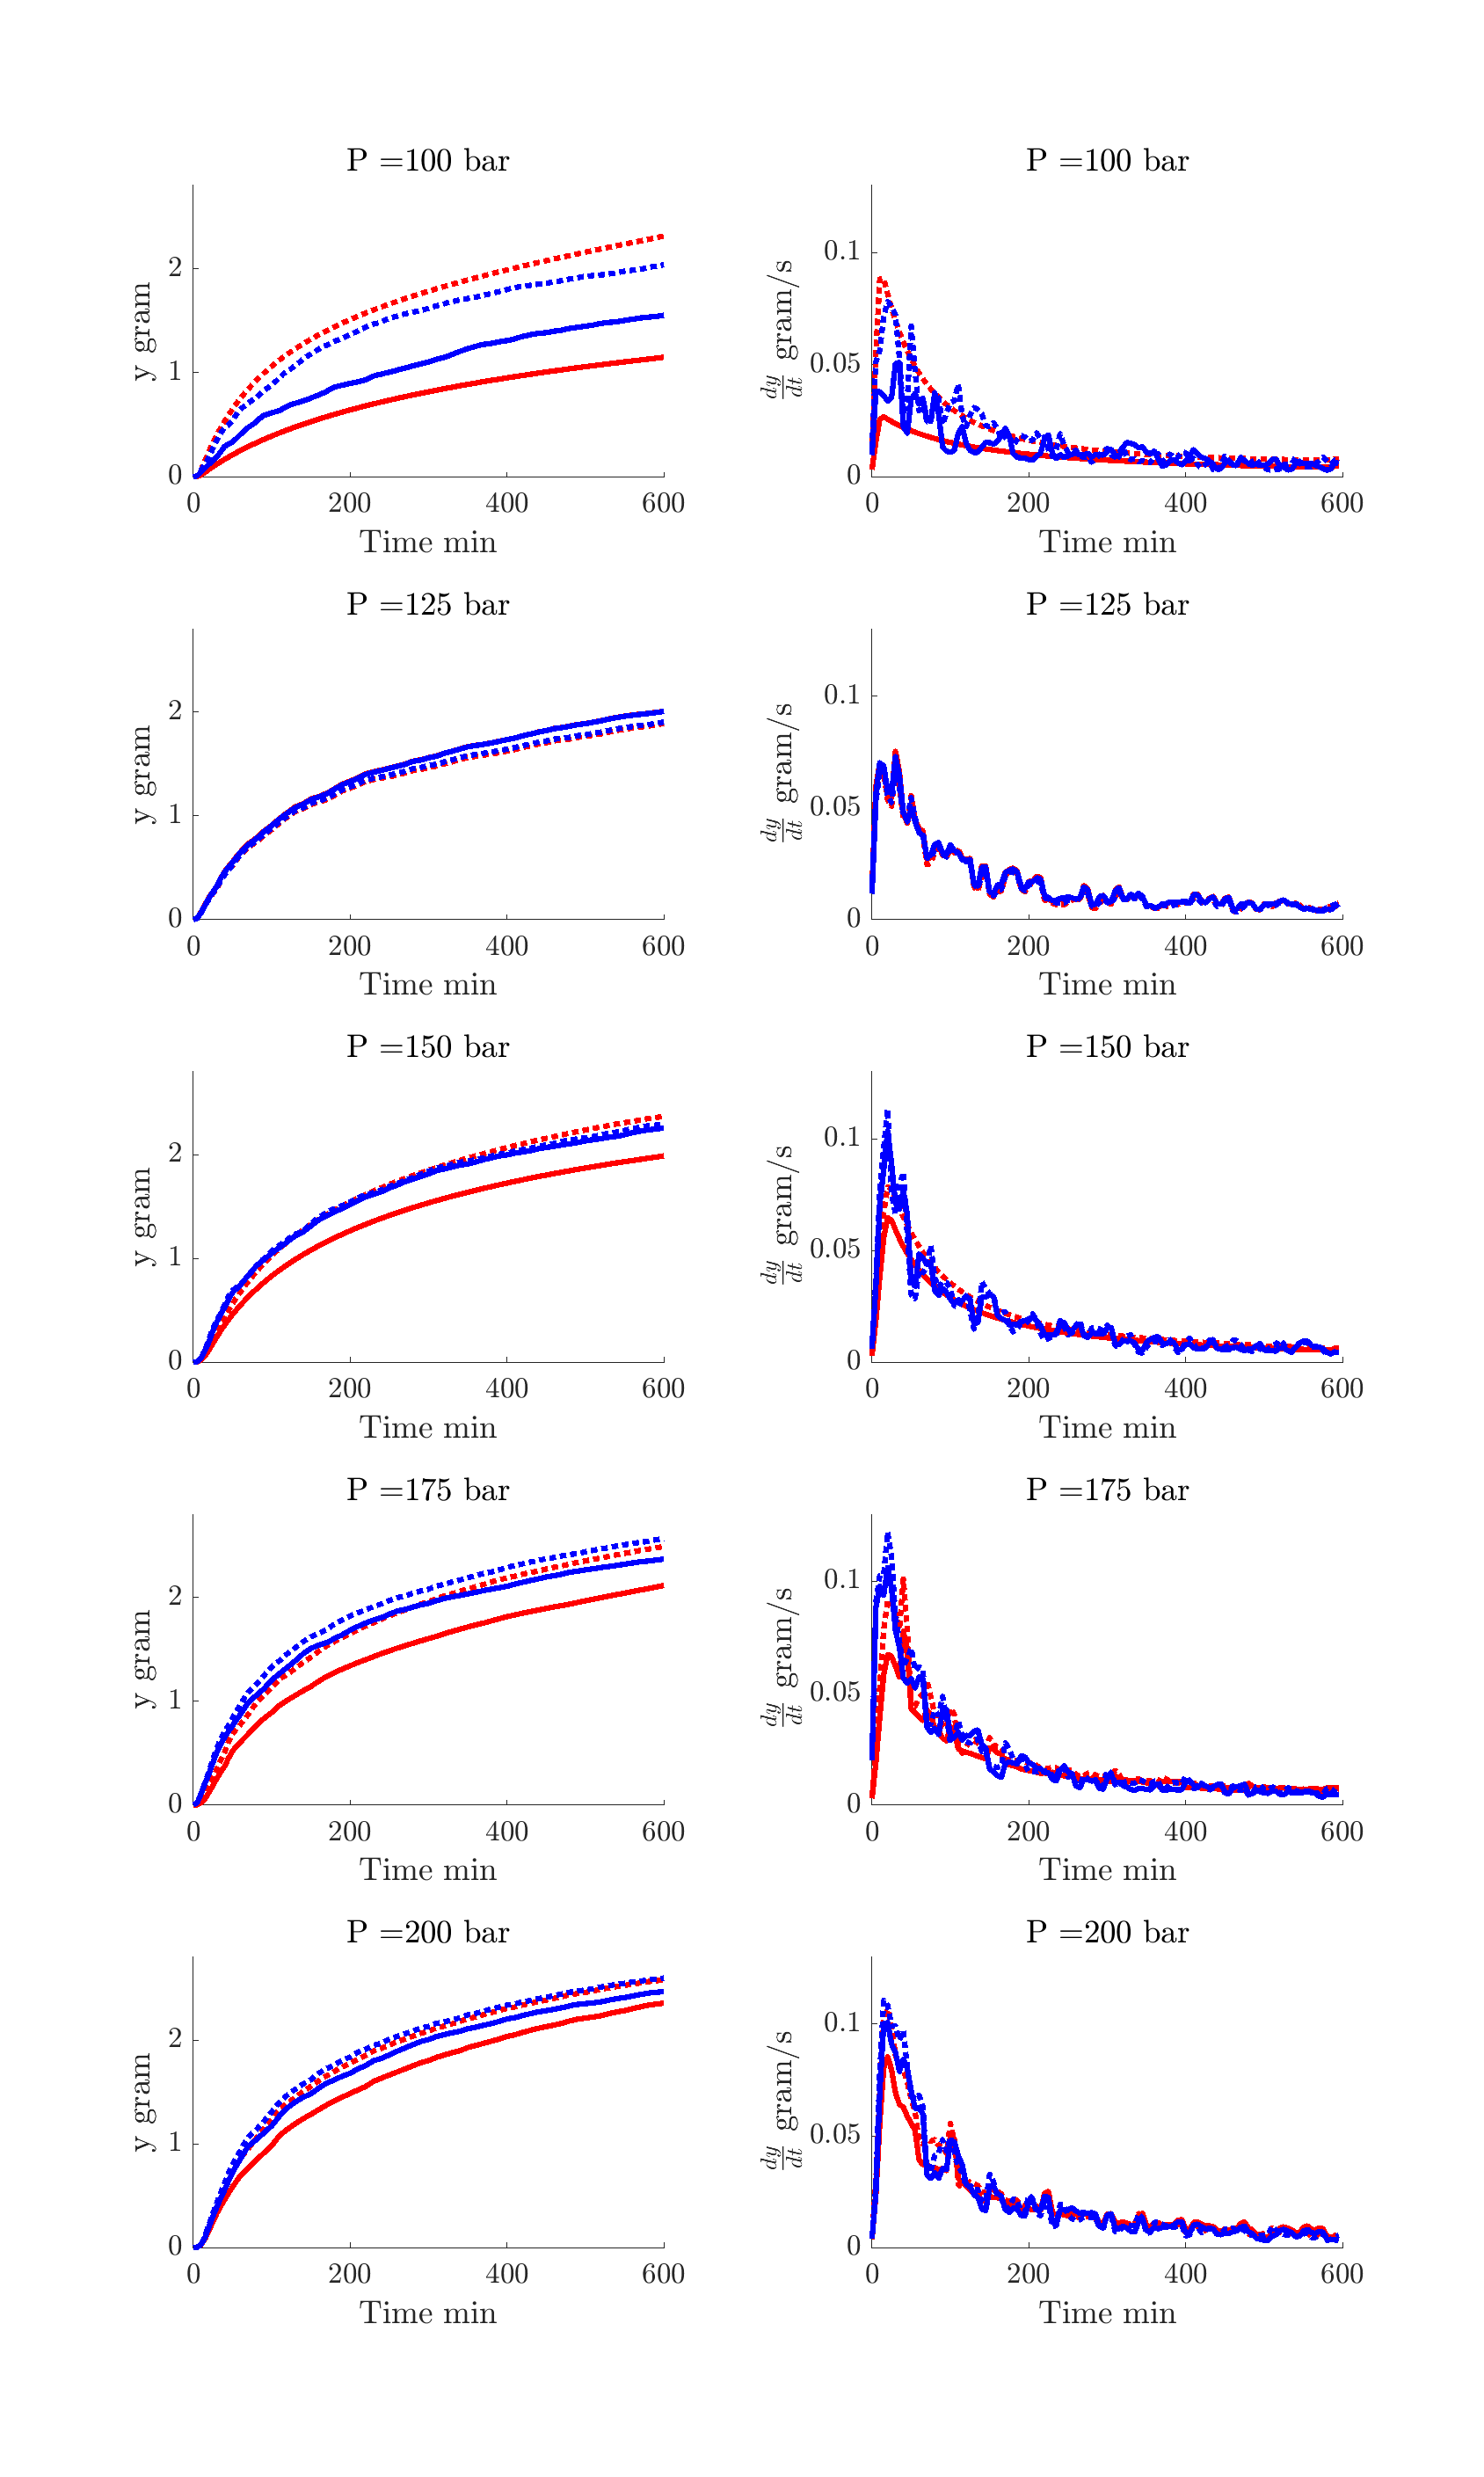
\includegraphics[trim= 2.5cm 2.5cm 2.2cm 2.5cm, clip, width=\columnwidth]{Figures/Results/Profiles_Y.png}	
		\caption{Yield profiles}
		\label{fig:Porfiles_Y}
	\end{figure}
	
\end{document}








































